%%
%% Automatically generated file from DocOnce source
%% (https://github.com/hplgit/doconce/)
%%

% #define PREAMBLE

% #ifdef PREAMBLE
%-------------------- begin preamble ----------------------

\documentclass[%
oneside,                 % oneside: electronic viewing, twoside: printing
final,                   % draft: marks overfull hboxes, figures with paths
10pt]{article}

\listfiles               %  print all files needed to compile this document

\usepackage{relsize,makeidx,color,setspace,amsmath,amsfonts,amssymb}
\usepackage[table]{xcolor}
\usepackage{bm,ltablex,microtype}

\usepackage[pdftex]{graphicx}

\usepackage[T1]{fontenc}
%\usepackage[latin1]{inputenc}
\usepackage{ucs}
\usepackage[utf8x]{inputenc}

\usepackage{lmodern}         % Latin Modern fonts derived from Computer Modern

% Hyperlinks in PDF:
\definecolor{linkcolor}{rgb}{0,0,0.4}
\usepackage{hyperref}
\hypersetup{
    breaklinks=true,
    colorlinks=true,
    linkcolor=linkcolor,
    urlcolor=linkcolor,
    citecolor=black,
    filecolor=black,
    %filecolor=blue,
    pdfmenubar=true,
    pdftoolbar=true,
    bookmarksdepth=3   % Uncomment (and tweak) for PDF bookmarks with more levels than the TOC
    }
%\hyperbaseurl{}   % hyperlinks are relative to this root

\setcounter{tocdepth}{2}  % levels in table of contents

% Tricks for having figures close to where they are defined:
% 1. define less restrictive rules for where to put figures
\setcounter{topnumber}{2}
\setcounter{bottomnumber}{2}
\setcounter{totalnumber}{4}
\renewcommand{\topfraction}{0.95}
\renewcommand{\bottomfraction}{0.95}
\renewcommand{\textfraction}{0}
\renewcommand{\floatpagefraction}{0.75}
% floatpagefraction must always be less than topfraction!
% 2. ensure all figures are flushed before next section
\usepackage[section]{placeins}
% 3. enable begin{figure}[H] (often leads to ugly pagebreaks)
%\usepackage{float}\restylefloat{figure}

\usepackage[framemethod=TikZ]{mdframed}

% --- begin definitions of admonition environments ---

% Admonition style "mdfbox" is an oval colored box based on mdframed
% "notice" admon
\definecolor{mdfbox_notice_background}{rgb}{1,1,1}
\newmdenv[
  skipabove=15pt,
  skipbelow=15pt,
  outerlinewidth=0,
  backgroundcolor=mdfbox_notice_background,
  linecolor=black,
  linewidth=2pt,       % frame thickness
  frametitlebackgroundcolor=mdfbox_notice_background,
  frametitlerule=true,
  frametitlefont=\normalfont\bfseries,
  shadow=false,        % frame shadow?
  shadowsize=11pt,
  leftmargin=0,
  rightmargin=0,
  roundcorner=5,
  needspace=0pt,
]{notice_mdfboxmdframed}

\newenvironment{notice_mdfboxadmon}[1][]{
\begin{notice_mdfboxmdframed}[frametitle=#1]
}
{
\end{notice_mdfboxmdframed}
}

% Admonition style "mdfbox" is an oval colored box based on mdframed
% "summary" admon
\definecolor{mdfbox_summary_background}{rgb}{1,1,1}
\newmdenv[
  skipabove=15pt,
  skipbelow=15pt,
  outerlinewidth=0,
  backgroundcolor=mdfbox_summary_background,
  linecolor=black,
  linewidth=2pt,       % frame thickness
  frametitlebackgroundcolor=mdfbox_summary_background,
  frametitlerule=true,
  frametitlefont=\normalfont\bfseries,
  shadow=false,        % frame shadow?
  shadowsize=11pt,
  leftmargin=0,
  rightmargin=0,
  roundcorner=5,
  needspace=0pt,
]{summary_mdfboxmdframed}

\newenvironment{summary_mdfboxadmon}[1][]{
\begin{summary_mdfboxmdframed}[frametitle=#1]
}
{
\end{summary_mdfboxmdframed}
}

% Admonition style "mdfbox" is an oval colored box based on mdframed
% "warning" admon
\definecolor{mdfbox_warning_background}{rgb}{1,1,1}
\newmdenv[
  skipabove=15pt,
  skipbelow=15pt,
  outerlinewidth=0,
  backgroundcolor=mdfbox_warning_background,
  linecolor=black,
  linewidth=2pt,       % frame thickness
  frametitlebackgroundcolor=mdfbox_warning_background,
  frametitlerule=true,
  frametitlefont=\normalfont\bfseries,
  shadow=false,        % frame shadow?
  shadowsize=11pt,
  leftmargin=0,
  rightmargin=0,
  roundcorner=5,
  needspace=0pt,
]{warning_mdfboxmdframed}

\newenvironment{warning_mdfboxadmon}[1][]{
\begin{warning_mdfboxmdframed}[frametitle=#1]
}
{
\end{warning_mdfboxmdframed}
}

% Admonition style "mdfbox" is an oval colored box based on mdframed
% "question" admon
\definecolor{mdfbox_question_background}{rgb}{1,1,1}
\newmdenv[
  skipabove=15pt,
  skipbelow=15pt,
  outerlinewidth=0,
  backgroundcolor=mdfbox_question_background,
  linecolor=black,
  linewidth=2pt,       % frame thickness
  frametitlebackgroundcolor=mdfbox_question_background,
  frametitlerule=true,
  frametitlefont=\normalfont\bfseries,
  shadow=false,        % frame shadow?
  shadowsize=11pt,
  leftmargin=0,
  rightmargin=0,
  roundcorner=5,
  needspace=0pt,
]{question_mdfboxmdframed}

\newenvironment{question_mdfboxadmon}[1][]{
\begin{question_mdfboxmdframed}[frametitle=#1]
}
{
\end{question_mdfboxmdframed}
}

% Admonition style "mdfbox" is an oval colored box based on mdframed
% "block" admon
\definecolor{mdfbox_block_background}{rgb}{1,1,1}
\newmdenv[
  skipabove=15pt,
  skipbelow=15pt,
  outerlinewidth=0,
  backgroundcolor=mdfbox_block_background,
  linecolor=black,
  linewidth=2pt,       % frame thickness
  frametitlebackgroundcolor=mdfbox_block_background,
  frametitlerule=true,
  frametitlefont=\normalfont\bfseries,
  shadow=false,        % frame shadow?
  shadowsize=11pt,
  leftmargin=0,
  rightmargin=0,
  roundcorner=5,
  needspace=0pt,
]{block_mdfboxmdframed}

\newenvironment{block_mdfboxadmon}[1][]{
\begin{block_mdfboxmdframed}[frametitle=#1]
}
{
\end{block_mdfboxmdframed}
}

% --- end of definitions of admonition environments ---

% prevent orhpans and widows
\clubpenalty = 10000
\widowpenalty = 10000

% --- end of standard preamble for documents ---


\usepackage[swedish]{babel}

\raggedbottom
\makeindex
\usepackage[totoc]{idxlayout}   % for index in the toc
\usepackage[nottoc]{tocbibind}  % for references/bibliography in the toc

%-------------------- end preamble ----------------------

\begin{document}

% matching end for #ifdef PREAMBLE
% #endif

\newcommand{\exercisesection}[1]{\subsection*{#1}}

% This file is to be run by preprocess to produce newcommands.tex
% to be included in .tex files.
% There are format-specific tests here for the newcommands (i.e.,
% different definitions of the commands depending on latex or mathjax).

% Newcommands for LaTeX math.
\newcommand{\tp}{\thinspace .}
\renewcommand{\Re}{\bbbr}
\newcommand{\Oof}[1]{\mathcal{O}(#1)}
\newcommand{\Prob}[1]{\hbox{P}(#1)}
\newcommand{\Var}[1]{\hbox{Var}(#1)}
\newcommand{\Cov}[2]{\hbox{Cov}(#1,#2)}
\newcommand{\StDev}[1]{\hbox{StDev}(#1)}

\newcommand{\punkt}{\thinspace .}
\newcommand{\komma}{\thinspace ,}

\newcommand{\vr}{\vec{r}}
\newcommand{\vrp}{\vec{r}\,'}
\newcommand{\erf}{\mathrm{erf}}
\newcommand{\vrho}{\vec{\varrho}}
\newcommand{\vrhop}{\vec{\varrho}\, '}
\newcommand{\sign}{\mathrm{sign}}

\newcommand{\Tr}[1]{\mathrm{Tr}[#1]}
\newcommand{\e}{\varepsilon}
\newcommand{\g}{\gamma}

\newcommand{\half}{\frac{1}{2}}
\newcommand{\vnabla}{\vec{\nabla}}


% Use footnotesize in subscripts
\newcommand{\subsc}[2]{#1_{\mbox{\footnotesize #2}}}




% ------------------- main content ----------------------



% ----------------- title -------------------------

\thispagestyle{empty}

\begin{center}
{\LARGE\bf
\begin{spacing}{1.25}
FFM234, Klassisk fysik och vektorfält - Föreläsningsanteckningar
\end{spacing}
}
\end{center}

% ----------------- author(s) -------------------------

\begin{center}
{\bf \href{{http://fy.chalmers.se/subatom/tsp/}}{Christian Forssén}, Institutionen för fysik, Chalmers, Göteborg, Sverige${}^{}$} \\ [0mm]
\end{center}

\begin{center}
% List of all institutions:
\end{center}
    
% ----------------- end author(s) -------------------------

% --- begin date ---
\begin{center}
Oct 1, 2018
\end{center}
% --- end date ---

\vspace{1cm}



\begin{summary_mdfboxadmon}[Repetition: Singulära fält]

\paragraph{Punktkälla i origo.}
\begin{itemize}
\item Fältet i punkten $\vec{r}$
\end{itemize}

\noindent
\begin{equation}
  \vec{F}(\vec{r}) = \frac{q}{4 \pi r^2} \hat{e}_r,
\end{equation}
fås av potentialen
\begin{equation}
  \phi(\vec{r}) = \frac{q}{4 \pi r},
\end{equation}
eftersom $\vec{F} = - \vnabla \phi$.

\begin{itemize}
\item Superposition ger potentialen i punkten $\vec{r}$ från en laddningsfördelning $\phi(\vec{r}) = \int \rho(\vec{r}\,') \frac{1}{4\pi|\vec{r} - \vec{r}\,'|} dV'$, där $G(\vec{r}, \vec{r}\,') \equiv \frac{1}{4\pi|\vec{r} - \vec{r}\,'|}$ kallas för Greensfunktionen i $\Bbb{R}^3$.

\item Hur skall vi skriva källtätheten, $\rho (\vec{r}) = \vnabla \cdot \vec{F}$, för en punktkälla? Och hur skall vi hantera Gauss sats?
\end{itemize}

\noindent
\begin{equation}
  \int_V \vnabla \cdot \vec{F} \mbox{d}V = \oint_{\partial V} \vec{F} \cdot \mbox{d} \vec{S},
\end{equation}
Vi har att $\vnabla \cdot \vec{F} = 0$ för $ r \neq 0 $,
men explicit uträkning ger $\mathrm{HL} = q$ om den inneslutna volymen $V$ innehåller origo.
\end{summary_mdfboxadmon} % title: Repetition: Singulära fält



\subsection*{7. Deltafunktioner}

Kan vi approximera $\vnabla \cdot \vec{F} = \rho (\vec{r})$, där laddningsfördelningen motsvarar en punktkälla, på något sätt? T.ex.
\begin{equation}
\rho_\varepsilon (\vec{r}) = \left\{
\begin{array}{ll}
c & r < \varepsilon \\ 
0 & r > \varepsilon
\end{array}
\right.
\end{equation}
Dvs, en ``utsmetad'' punktladdning där vi väljer $c$ så att den totala laddningen är $q$, dvs
\begin{equation}
\rho_\varepsilon (\vec{r}) = \left\{
\begin{array}{ll}
\frac{q}{4\pi\varepsilon^3/3} & r \le \varepsilon \\ 
0 & r > \varepsilon
\end{array}
\right.
\end{equation}
\begin{itemize}
\item Vad blir funktionen då $\varepsilon \to 0^+$? 

\item Det kan vi tyvärr inte definiera.

\item $\rho(\vec{r}) = \lim_{\varepsilon \to 0^+} \rho_\varepsilon(\vec{r})$ är inte en funktion; sekvensen av funktioner som erhålls genom att variera $\varepsilon$ kallas för en distribution.
\end{itemize}

\noindent
\subsection*{Deltafunktioner i en dimension}

\paragraph{Punktkälla i $D=1$.}
I en dimension kan vi definiera en punktkälla från potentialen
\begin{equation}
\phi(x) = -\frac{q}{2} \left| x \right|
\end{equation}



\vspace{6mm}

% inline figure
\centerline{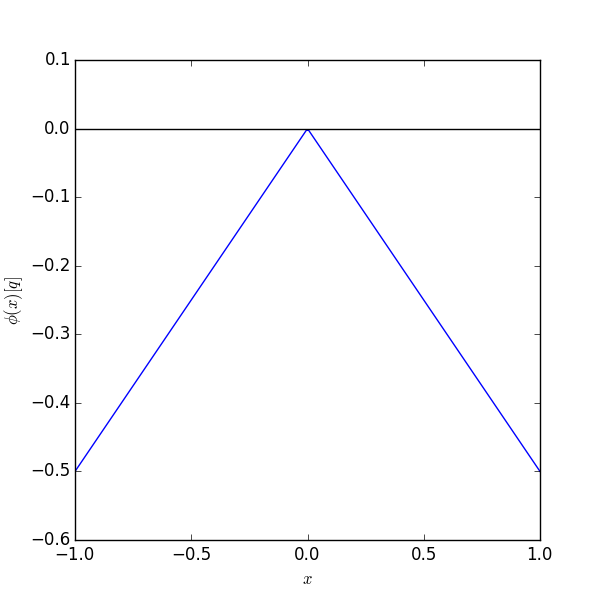
\includegraphics[width=0.7\linewidth]{fig/pointcharge_pot_1dim.png}}

\vspace{6mm}



vilket ger fältet
\begin{equation}
\vec{F}(x) = -\hat{x} \frac{\mbox{d}\phi}{\mbox{d}x} = 
\left\{
\begin{array}{ll}
\frac{q}{2} \hat{x} & x > 0 \\ 
-\frac{q}{2} \hat{x} & x < 0 \\ 
\end{array}
\right.
\end{equation}



\vspace{6mm}

% inline figure
\centerline{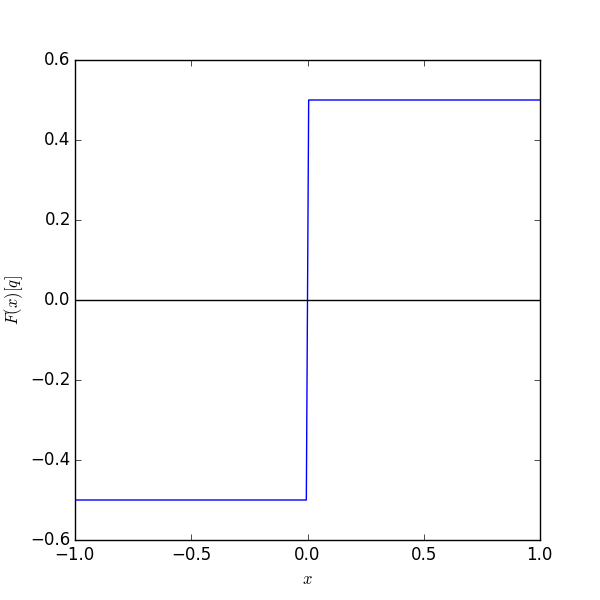
\includegraphics[width=0.7\linewidth]{fig/pointcharge_field_1dim.png}}

\vspace{6mm}



Vi kallar den enda komponenten av detta vektorfält för $F(x)$, dvs $F(x) = \frac{q}{2}\sign(x)$. Motsvarigheten till Gauss sats för detta endimensionella fält är 
\begin{equation}
\int_a^b \frac{dF}{dx} dx  = F(b) - F(a) = 
\left\{
\begin{array}{ll}
q, & \mathrm{om~} a < 0 < b \\ 
0, & \mathrm{annars} \\ 
\end{array}
\right.
\end{equation}
medan en naiv insättning av $\mbox{d}F / \mbox{d}x = 0$ i VL hade gett noll.

Problemet är ju att $\frac{dF}{dx} = 0$ för $x \neq 0$, men ``$\frac{dF}{dx} =  \infty$'' för $x = 0$. Vi kan uttrycka detta som en ``funktion'', $\frac{dF}{dx} = q \delta(x)$, där
\begin{itemize}
\item $\delta(x)$ är noll då $x \neq 0$, och

\item integralen $\int_{a<0}^{b>0} \delta(x) \mbox{d}x = 1$.
\end{itemize}

\noindent
\paragraph{Distributioner.}
Vi konstruerar denna ``funktion'' som en gräns $\varepsilon \to 0^+$ för distributionen
\begin{equation}
h_\varepsilon(x)
= \left\{
\begin{array}{ll}
0 & |x| > \frac{\varepsilon}{2} \\ 
\frac{1}{\varepsilon} & |x| < \frac{\varepsilon}{2} \\ 
\end{array}
\right.
\end{equation}



\vspace{6mm}

% inline figure
\centerline{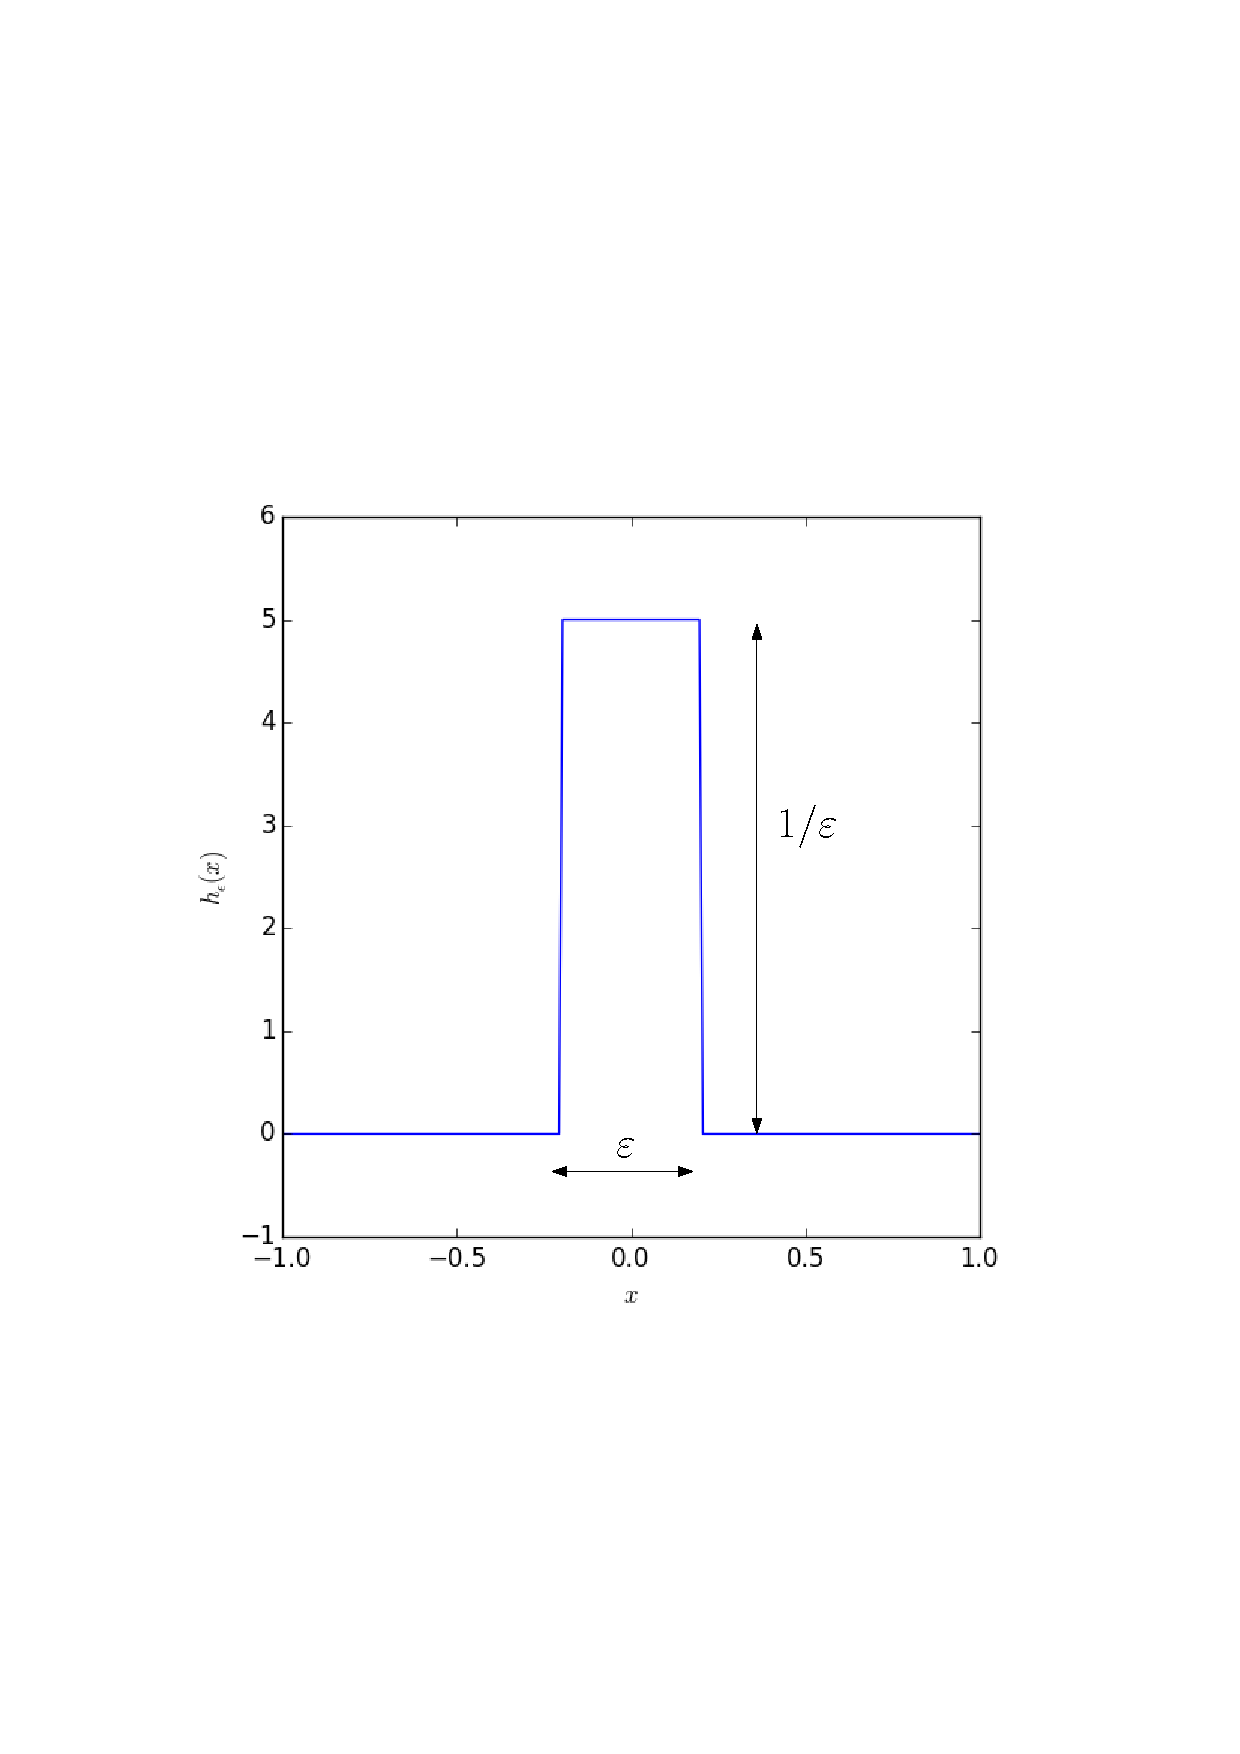
\includegraphics[width=0.7\linewidth]{fig/delta_step.pdf}}

\vspace{6mm}



\paragraph{Kontrollera.}
$$
\lim_{\varepsilon \to 0} h_\varepsilon(x) = 0,
$$
för $x \neq 0$. Dessutom har vi
$$
\lim_{\varepsilon \to 0} \int_{a<0}^{b>0} h_\varepsilon(x) \mbox{d}x 
= \lim_{\varepsilon \to 0} \int_{-\varepsilon/2}^{\varepsilon/2} \frac{1}{\varepsilon} \mbox{d}x = \lim_{\varepsilon \to 0} \frac{1}{\varepsilon} \left[ x \right]_{-\varepsilon/2}^{\varepsilon/2}
= \lim_{\varepsilon \to 0} 1 = 1.
$$
---------------------------------------

Men det finns också andra möjligheter:
\begin{align}
h_\varepsilon(x) &= \frac{\exp(-x^2 / \varepsilon^2)}{\sqrt{\pi} \varepsilon}, \\ 
h_\varepsilon(x) &= \frac{\varepsilon}{\pi (x^2 + \varepsilon^2)}, \\ 
h_\varepsilon(x) &= \frac{\sin(x/\varepsilon)}{\pi x} \label{eq:sinxdelta}.
\end{align}




\vspace{6mm}

% inline figure
\centerline{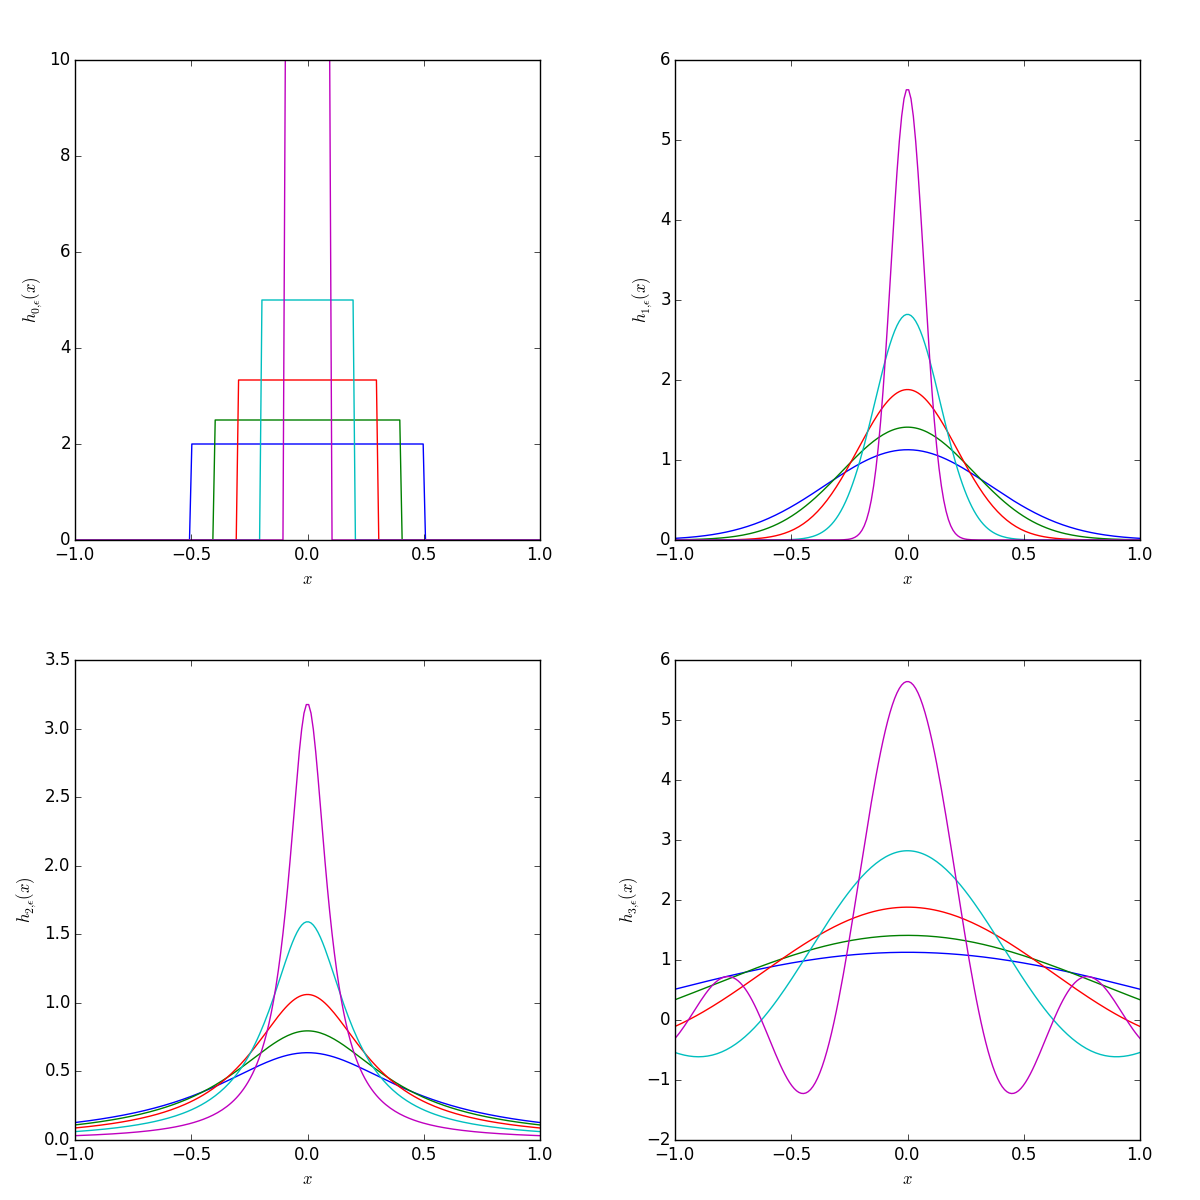
\includegraphics[width=0.95\linewidth]{fig/deltas.png}}

\vspace{6mm}



Samtliga dessa utgör en \emph{sekvens av funktioner} (en \emph{distribution}) från vilka vi kan definiera \emph{Diracs deltafunktion}
\begin{equation}
\delta(x) = \lim_{\varepsilon \to 0^+} h_\varepsilon(x)
\end{equation}
med de definierande egenskaperna

\begin{block_mdfboxadmon}[]
\begin{align}
\delta(x) &= 0, \quad x \neq 0 \\ 
f(0) &= \int_a^b f(x) \delta(x) \mbox{d}x,
\end{align}
där $f(x)$ är en välbeteende funktion och $\left[ a,b \right]$ inkluderar 0.
\end{block_mdfboxadmon} % title: 



Ett specialfall ($f(x)=1$) av ovanstående är
\begin{equation}
\int_{-\infty}^{+\infty} \delta(x) \mbox{d}x = 1
\end{equation}

------------------------------


\begin{notice_mdfboxadmon}[Exempel: endimensionella deltafunktioner]

Kontrollera att vi erhåller Diracs deltafunktion från sekvensen $h_\varepsilon(x) = \frac{\exp(-x^2 / \varepsilon^2)}{\sqrt{\pi} \varepsilon}$.

\emph{Lösning}:
För $x \neq 0$ gäller
\begin{align}
h_\varepsilon(x) 
&= \frac{1}{\sqrt{\pi} \varepsilon \exp(x^2 / \varepsilon^2)}
= \frac{1}{\sqrt{\pi} \varepsilon \left[ 1 + \frac{x^2}{\varepsilon^2} + \frac{1}{2}\left(\frac{x^2}{\varepsilon^2}\right)^2 + \ldots \right] } \nonumber \\ 
&= \frac{\varepsilon}{\sqrt{\pi}} \frac{1}{\left( x^2 + \varepsilon^2 + \frac{x^4}{2\varepsilon^2} + \ldots \right)} \to 0 \quad \mathrm{då~} \varepsilon \to 0^+
\label{eq:heps0}
\end{align}
Vidare har vi integralen $\int_{-\infty}^\infty e^{-x^2 / \varepsilon^2} \mbox{d}x = \sqrt{\pi \varepsilon^2}$ (se tabell över definita integraler, eventuellt Beta 7.5-41). Detta ger
\begin{equation}
\lim_{\varepsilon \to 0^+}
\int_{-\infty}^{+\infty} \frac{\exp(-x^2 / \varepsilon^2)}{\sqrt{\pi} \varepsilon} \mbox{d}x = \lim_{\varepsilon \to 0} \frac{\sqrt{\pi \varepsilon^2}}{\sqrt{\pi} \varepsilon} = 1, \quad \mathrm{för~} \varepsilon>0.
\label{eq:heps1}
\end{equation}
För att vara helt korrekta skall vi egentligen visa den mer allmänna egenskapen $\int_a^b f(x) \delta(x) \mbox{d}x = f(0)$ för en väl beteende funktion $f(x)$. Eftersom ekv. (\ref{eq:heps0}) gäller, och $f(x)$ inte utgör något problem, kan vi utöka integrationsintervallet och istället studera
\begin{equation}
\int_{-\infty}^{+\infty} f(x) \delta(x) \mbox{d}x = f(0).
\end{equation}
Vi Taylorutvecklar, $f(x) = f(0) + f'(0)x + f''(0)x^2/2+\ldots$, och konstaterar att 

\begin{equation}
\lim_{\varepsilon \to 0} \int_{-\infty}^{+\infty} f(0) h_\varepsilon(x) \mbox{d}x = f(0) \lim_{\varepsilon \to 0} \int_{-\infty}^{+\infty} h_\varepsilon(x) \mbox{d}x = f(0),
\end{equation}
enligt vad vi visat ovan (\ref{eq:heps1}). Det återstår att visa att 
\begin{equation}
\lim_{\varepsilon \to 0} \int_{-\infty}^{+\infty} x^n h_\varepsilon(x) \mbox{d}x = 0,
\label{eq:xnheps0}
\end{equation}
för alla heltal $n>0$. I vårt fall har vi en jämn funktion $h_\varepsilon(x)$ vilket gör att ekv. (\ref{eq:xnheps0}) är trivialt uppfyllt för udda $n$ då integranden blir udda. För jämna $n=2k$ finner vi (se t.ex. Beta 7.5-42) 
\begin{equation}
\lim_{\varepsilon \to 0^+}
\int_{-\infty}^{+\infty} x^{2k} \frac{\exp(-x^2 / \varepsilon^2)}{\sqrt{\pi} \varepsilon} \mbox{d}x = \lim_{\varepsilon \to 0} \frac{2}{\sqrt{\pi} \varepsilon} \frac{(2k-1)!!}{2^{k+1}} \sqrt{\pi} \varepsilon \varepsilon^{2k} = 0.
\end{equation}
Alltså har vi visat att
\begin{equation}
\lim_{\varepsilon \to 0^+}
\int_{a<0}^{b>0} f(x) \frac{\exp(-x^2 / \varepsilon^2)}{\sqrt{\pi} \varepsilon} \mbox{d}x = f(0), \quad \mathrm{för~} \varepsilon>0.
\end{equation}
\end{notice_mdfboxadmon} % title: Exempel: endimensionella deltafunktioner



\subsection*{Egenskaper hos Diracs deltafunktion}

\begin{itemize}
\item Jämn: $$\delta(-x) = \delta(x)$$

\item Skalning: 
\end{itemize}

\noindent
$$
\delta(ax) = \frac{1}{|a|} \delta(x).
$$ 


\begin{warning_mdfboxadmon}[Kommentar]
Visas enklast genom att göra substitutionen $y=x a$ i uttrycket 
$$
\int_{-\infty}^{+\infty} f(x) \delta(ax) \mbox{d}x.
$$ 
Var noga med tecknet på integrationsgränserna.
\end{warning_mdfboxadmon} % title: Kommentar


\begin{itemize}
\item Translation: 
\end{itemize}

\noindent
$$
\int_{-\infty}^{+\infty} f(x) \delta(x-x_0) \mbox{d}x = f(x_0).
$$

\begin{warning_mdfboxadmon}[Kommentar]
visas genom substitutionen $y=x-x_0$.
\end{warning_mdfboxadmon} % title: Kommentar


\begin{itemize}
\item Derivata 
\end{itemize}

\noindent
$$
\int_{-\infty}^{+\infty} f(x) \delta'(x-x_0) \mbox{d}x = -\int_{-\infty}^{+\infty} f'(x) \delta(x-x_0) \mbox{d}x = -f'(x_0),
$$
vilket kan betraktas som definitionen av derivatan $\delta'(x)$.


\begin{warning_mdfboxadmon}[Kommentar]
Visas genom partiell integration med någon av funktionssekvenserna som definierar deltafunktionen.
\end{warning_mdfboxadmon} % title: Kommentar


\begin{itemize}
\item Kan generaliseras till fler dimensioner. Vi skriver generellt $\delta^{(D)}(\vec{r})$, där vi skall tolka superskriptet som antalet dimensioner. T.ex. har vi för $D=3$ 
\end{itemize}

\noindent
$$
\delta^{(3)}(\vec{r}) = \delta(x) \delta(y) \delta(z).
$$
I sfäriska koordinater blir detta
$$
\iiint f(\vec{r}) \delta^{(3)}(\vec{r} - \vec{r}_0) r^2 \sin\theta \mbox{d}r \mbox{d}\theta \mbox{d}\phi = f(\vec{r}_0).
$$
Med vissa förbehåll (se t.ex. upp för punkten $\vec{r}_0=0$ i sfäriska koordinater) kan deltafunktionen i kroklinjiga koordinater skrivas
$$
\delta^{(3)}(\vec{r} - \vec{r}_0) = \frac{1}{h_1(\vec{r}_0) h_2(\vec{r}_0) h_3(\vec{r}_0)} \delta(u_1-u_{1,0}) \delta(u_2-u_{2,0}) \delta(u_3-u_{3,0}).
$$


\begin{warning_mdfboxadmon}[Rita]
Skissa gärna den ``primitiva funktionen'' till en deltafunktion i en dimension.
\end{warning_mdfboxadmon} % title: Rita



\subsection*{Deltafunktioner i högre dimensioner}

Vi startar med punktkällan i origo: $\vec{F} = \frac{q}{4 \pi r^2} \hat{e}_r$, och den problematiska volymsintegralen
$$
\int_V \vnabla \cdot \vec{F} \mbox{d}V,
$$
som borde bli lika med $q$ om $V$ omfattar origo. Detta kan vi åstadkomma genom att införa $\vnabla \cdot \vec{F} = q \delta^3(x) = q \delta(x)\delta(y)\delta(z)$ eftersom
$$
\int_V \delta(x)\delta(y)\delta(z) \mbox{d}x \mbox{d}y \mbox{d}z = 1.
$$
Låt oss använda sfäriska koordinater. Hur kan vi uttrycka $\delta^{(3)}(\vec{r})$ så att följande integralegenskap uppfylls?
$$
\int_V \delta^{(3)}(\vec{r}) r^2 \sin\theta dr d\theta d\varphi = 1,
$$
om volymen $V$ innesluter origo. Vi vill finna $\delta^{(3)}(\vec{r})$ som ett gränsvärde av en distribution $h_\varepsilon(\vec{r})$.

Starta från ett \emph{regulariserat} fält
\begin{equation}
\vec{F}_\varepsilon(\vec{r}) = \frac{q}{4 \pi (r^2 + \varepsilon^2)} \hat{e}_r
\end{equation}
som uppenbarligen går mot $\vec{F}$ då $\varepsilon \to 0^+$.

Divergensen för $r \neq 0$ blir ($\vnabla \cdot \vec{F} = \frac{1}{r^2} \frac{\partial}{\partial r} (r^2 F_r) + \ldots$)
\begin{equation}
\vnabla \cdot \vec{F}_\varepsilon(\vec{r}) = \frac{q}{4 \pi r^2} \underbrace{\frac{\partial}{\partial r} \left( \frac{r^2}{r^2 + \varepsilon^2} \right)}_{=\frac{2r}{r^2 + \varepsilon^2} - \frac{2 r r^2}{(r^2 + \varepsilon^2)^2} = \frac{2 r \varepsilon^2}{(r^2 + \varepsilon^2)^2}}
= \frac{q \varepsilon^2}{2 \pi} \frac{1}{r(r^2 + \varepsilon^2)^2} \to 0 \quad \mathrm{då} \; \varepsilon \to 0.
\end{equation}
Utan styrkan $q$ kallar vi denna sekvens av funktioner för $h_\varepsilon(\vec{r})$ och påstår att $\lim_{\varepsilon \to 0} h_\varepsilon(\vec{r}) = \delta^3(\vec{r})$. Utför integralen
\begin{align}
\int_V \vnabla \cdot \vec{F}_\varepsilon \mbox{d} V &= \int_V q h_\varepsilon(\vec{r}) \mbox{d} V = \frac{ q \varepsilon^2}{2 \pi} 4\pi \int_0^\infty r^2 \mbox{d} r \frac{1}{r(r^2 + \varepsilon^2)^2} \\ 
&= 2 q \varepsilon^2 \left[ -\frac{1}{2} \frac{1}{r^2 + \varepsilon^2} \right]_0^\infty = 2 q \varepsilon^2 \frac{1}{2 \varepsilon^2} = q
\end{align}
Alltså har vi visat att
\begin{itemize}
\item $\lim_{\varepsilon \to 0} h_\varepsilon(\vec{r}) = 0$ för $r \neq 0$.

\item $\int_{\mathbf{R}^3} h_\varepsilon(\vec{r}) \mbox{d}V = 1$
\end{itemize}

\noindent
Alltså skriver vi källtätheten 
$$
\rho(\vec{r}) = \vnabla \cdot \vec{F} = -\Delta \phi = q \delta^3(\vec{r}).
$$

\paragraph{Linjekälla.}
Linjekällan $\vec{F} = \frac{k}{2 \pi \rho} \hat{e}_\rho$ (motsvarar en punktkälla i $D=2$).
Källtätheten kan skrivas
$$
\vnabla \cdot \vec{F} = k \delta^2(\vec{\rho}) \left( = k \delta(x) \delta(y) \right).
$$
Studera t.ex. normalytintegralen genom en cylinder med höjden $L$ runt linjekällan
$$
\int_S \vec{F} \cdot \mbox{d}\vec{S} = \int_{S+S_0+S_L} \vec{F} \cdot \mbox{d}\vec{S} = \int_V \vnabla \cdot \vec{F} \mbox{d} V = \int_0^L \mbox{d} z \int \mbox{d}x \mbox{d}y k \delta(x)\delta(y) = \int_0^L \mbox{d} z k = k L.
$$
där vi först har slutit ytan genom att införa ytorna $S_0$ och $S_L$ som är cirkelskivor vid botten och toppen och som har normalytintegralen noll eftersom fältet är vinkelrät mot normalen.

\paragraph{Virveltråd.}
Vi kan resonera på liknande sätt för en virveltråd $\vec{F} = \frac{J}{2 \pi \rho} \hat{e}_\phi$. Stokes sats säger att
$$
\int_{\partial S} \vec{F} \cdot \mbox{d} \vec{r} = \int_S (\vnabla \times \vec{F}) \cdot \mbox{d} \vec{S},
$$
där vi kan räkna ut $\mathrm{VL} = J$ (t.ex. för en cirkel runt virveltråden). För detta fält är det rotationen som är problematisk. Notera att detta är en vektor.
$$
\vnabla \times \vec{F} = J \delta^2(\vec{\rho}) \hat{z} = \vec{J} \delta(x)\delta(y).
$$


\begin{notice_mdfboxadmon}[Avancerat exempel: tillämpning av deltafunktionen; Fouriertransform och ortogonalitet.]

Givet en funktion $f(x)$ definieras dess Fouriertransform som
$$
\tilde f(k)=\frac{1}{\sqrt{2\pi}}\int_{-\infty}^\infty dx\,e^{-ikx}f(x)
$$
Den inversa transformen ger frekvenssönderläggningen av $f(x)$, i detta fall motsvaras ``frekvensen'' av vågtalet $k$:
$$
f(x)=\frac{1}{\sqrt{2\pi}}\int_{-\infty}^\infty dk\,e^{ikx}\tilde f(k)
$$
(normeringen har valts för att åstadkomma symmetri mellan de två uttrycken).

Genom att sätta in det första uttrycket i det andra får man, under förutättning att man kan byta integrationsordning,
\begin{align*}
f(x)&=\frac{1}{2\pi}\int_{-\infty}^\infty dk\,e^{ikx}
\int_{-\infty}^\infty dx'\,e^{-ikx'}f(x') \\ 
&=
\frac{1}{2\pi}\int_{-\infty}^\infty dx'
\left(\,\int_{-\infty}^\infty dk\,e^{ik(x-x')}\right)f(x')
\end{align*}

Uttrycket inom parenteser i det sista ledet beror bara på $x-x'$, och om resultatet skall bli $f(x)$ måste det vara en deltafunktion lika med $2\pi\delta(x-x')$. Dvs
\begin{equation}
\delta(x-x') = \frac{1}{2\pi} \int_{-\infty}^\infty dk\,e^{ik(x-x')}.
\label{eq:expdelta}
\end{equation}
Genom att byta vågtalet $k$ och koordinaten $x$ får man också $2\pi \delta(k-k') = \int_{-\infty}^\infty dx\,e^{i(k-k')x}$. Detta sätt att skriva deltafunktionen kunde vi också ha anat från ekv. (\ref{eq:sinxdelta}) genom att byta 
$$
\lim_{\varepsilon \to 0} \frac{\sin(x/\varepsilon)}{\pi x} \Rightarrow \lim_{n \to \infty} \frac{\sin(n x)}{\pi x}.
$$
Här kan man nämligen göra omskrivningen
\begin{equation}
\int_{-n}^n e^{i x k} dk = \left[ \frac{e^{ixk}}{ix} \right]_{-n}^n 
= \left[ \frac{\cos(xk)+i\sin(xk)}{ix} \right]_{-n}^n 
= 2 \frac{\sin(nx)}{x},
\end{equation}
så att vi får
\begin{equation}
\delta(x) = \lim_{n \to \infty} \frac{1}{2\pi} \int_{-n}^n e^{i x k} dk,
\end{equation}
vilket är analogt med ekv. (\ref{eq:expdelta})

Funktionerna $e_k(x)=\frac{1}{\sqrt{2\pi}}e^{ikx}$ kan alltså ses som ortogonala och ``deltafunktionsnormerade'' med ortogonalitetsrelationen
$$
\int_{-\infty}^\infty dx\,e^{\mathstrut}_k(x)e^*_{k'}(x)=\delta(k-k')
$$

Man kan bekräfta resultatet genom att göra beräkningen explicit 
för de regulariserade funktionerna $e_{k,\varepsilon}(x)={1\over\sqrt{2\pi}}e^{ikx-\varepsilon^2x^2}$ och låta $\varepsilon\rightarrow0$ (se uppgift 7.15).
\end{notice_mdfboxadmon} % title: Avancerat exempel: tillämpning av deltafunktionen; Fouriertransform och ortogonalitet.



% ------------------- end of main content ---------------

% #ifdef PREAMBLE
\end{document}
% #endif

